% Document class `report-template` accepts either project-plan or final-report option in
% []. This will change the title page as necessary.
\documentclass[project-plan]{report-template}
% \documentclass[final-report]{report-template}

% Packages I use in my report.
\usepackage{graphicx}
\usepackage{amsmath}
\usepackage{amsfonts}
\usepackage{booktabs}
\usepackage{algorithm}
\usepackage{algorithmic}

% Directory where I saved my figures.
\graphicspath{{./figures/}}

% Metadata used for the title page - please modify.
\university{Imperial College London}
\department{Department of Earth Science and Engineering}
\course{MSc in Applied Computational Science and Engineering}
\title{Cognitive-Enhanced Knowledge Tracing: A Unified Framework Integrating LLM Semantics, Adaptive Forgetting, and Mixture-of-Experts}
\author{Yilin Jing}
\email{yilin.jing24@imperial.ac.uk}
\githubusername{yj1024}
\supervisors{Ms. Wenxia Yang\\
             Dr. Simon Warder}
\repository{https://github.com/ese-ada-lovelace-2024/irp-yj1024}

\begin{document}

\maketitlepage  % generate title page

% Academic Integrity Declaration
\section*{Academic Integrity Declaration}
I confirm that I have read, understood, and will comply with the IRP Academic Integrity requirements as outlined in the official guidelines. This project plan represents my own work, understanding, and academic effort. I acknowledge that:

\begin{itemize}
    \item All submitted work must be my own and reflect my personal knowledge and technical skills
    \item I will maintain regular version control with meaningful commits throughout the project
    \item I will attend all scheduled meetings with supervisors and maintain a detailed logbook
    \item Any use of external resources, including code, literature, or AI tools, will be properly cited and disclosed
    \item I understand that I may be required to defend this work in a viva or authenticity interview
\end{itemize}

I commit to upholding the highest standards of academic integrity throughout this Independent Research Project.

% AI Acknowledgement Statement
\subsection*{AI Acknowledgement Statement}
No generative AI tools were used in the preparation of this project plan. All content, ideas, and written work represent my own understanding and effort.
% Abstract
\newpage

\section*{Abstract}
Despite recent advances in educational AI, particularly the Knowledge Modeling and Material Prediction (KMaP) framework \cite{hashemifar2025personalized}, current systems struggle with three fundamental limitations: inadequate semantic understanding of educational content, oversimplified knowledge forgetting models, and static student profiling approaches. This project proposes a novel enhanced KMaP framework that addresses these limitations through three key innovations: (1) Large Language Model (LLM) semantic embeddings using sentence-BERT to capture rich conceptual relationships in learning materials, (2) adaptive time-decay gating mechanisms that model personalized knowledge forgetting patterns based on cognitive science principles \cite{sha2024forgetting,wang2024personalized}, and (3) a gated Mixture-of-Experts (MoE) architecture for dynamic student profiling that adapts to evolving learning behaviors \cite{li2025tutorllm,zou2025multi}. Our approach targets measurable improvements on the EdNet dataset \cite{choi2020ednet}: a minimum 1.5 percentage points (pp) enhancement in Mean Reciprocal Rank (MRR) and a 1 pp improvement in early-stage Area Under Curve (AUC) compared to baseline KMaP. This work represents a significant advancement in personalized educational technology by bridging cognitive science theories with modern deep learning architectures.


% Problem Description
\section{Introduction}

Online education has experienced unprecedented growth, but "one-size-fits-all" approaches lead to high dropout rates \cite{siemens2013learning}. Personalized learning, powered by Knowledge Tracing (KT), aims to solve this by modeling student knowledge states over time. The field has evolved from early Bayesian models (BKT) \cite{corbett1994knowledge} to deep learning architectures like DKT \cite{piech2015deep}, DKVMN \cite{zhang2017dynamic}, and attention-based models such as SAKT \cite{pandey2019self} and AKT \cite{ghosh2020context}, which leverage Transformer architectures \cite{vaswani2017attention}.

The current state-of-the-art is the Knowledge Modeling and Material Prediction (KMaP) framework \cite{hashemifar2025personalized}, which excels at simultaneously modeling knowledge and predicting learning materials. Despite its strengths, our analysis reveals three critical gaps that limit its effectiveness, leading to suboptimal learning outcomes:

\begin{itemize}
    \item \textbf{Semantic Representation Gap:} KMaP uses traditional embeddings that fail to capture rich semantic relationships between learning materials (e.g., "linear equations" vs. "algebraic expressions"). This limits recommendation accuracy for conceptually similar but presentationally different content, causing the system to miss valuable learning opportunities.
    \item \textbf{Oversimplified Forgetting Mechanisms:} The model lacks a sophisticated model of knowledge forgetting, a key cognitive principle \cite{ebbinghaus1885memory}. It uses fixed temporal dynamics, ignoring individual differences in memory retention, which affects long-term prediction quality and fails to schedule reviews effectively, particularly for students with irregular study patterns.
    \item \textbf{Static Student Profiling:} KMaP's student profiles are static. They are established once and do not adapt to a learner's evolving behaviors, preferences, and cognitive states over time. This rigidity prevents the system from responding to changes in a student's learning strategies or engagement levels.
\end{itemize}

To address these limitations, this research makes three novel contributions to educational AI. We introduce: (1) \textbf{LLM-Enhanced Content Representation} using sentence-BERT \cite{reimers2019sentence} to capture deep semantic meaning; (2) \textbf{Cognitive-Inspired Adaptive Forgetting} via personalized time-decay gates based on cognitive science \cite{wixted2004psychology,sha2024forgetting}; and (3) \textbf{Dynamic Student Profiling} with a gated Mixture-of-Experts (MoE) architecture \cite{fedus2022switch,shelhamer2022mixture} that adapts to evolving learning behaviors. Our work pioneers the integration of these modern techniques into a unified KT framework, aiming to create a more effective and truly personalized learning experience.

% Objectives
\section{Research Objectives and Success Criteria}

\subsection{Research Objectives}
This project aims to enhance the KMaP framework through three specific, measurable objectives:

\textbf{Objective 1: Semantic Enhancement}
\begin{itemize}
    \item Integrate sentence-BERT embeddings for material representation.
    \item Improve semantic similarity capture by 8-12\%.
    \item Validate conceptual modeling via similarity analysis.
\end{itemize}

\textbf{Objective 2: Adaptive Forgetting Implementation}
\begin{itemize}
    \item Develop personalized time-decay gating mechanisms.
    \item Improve long-term knowledge prediction accuracy by 5-10\%.
    \item Validate forgetting patterns against psychological models.
\end{itemize}

\textbf{Objective 3: Dynamic Student Profiling}
\begin{itemize}
    \item Implement a gated Mixture-of-Experts architecture.
    \item Improve capture of behavioral evolution by 10-15\%.
    \item Enable real-time profile adaptation to context changes.
\end{itemize}

\subsection{Quantitative Success Criteria}
Building upon KMaP's baseline performance, we target specific improvements on the EdNet dataset \cite{choi2020ednet}:

\begin{itemize}
    \item \textbf{Material Recommendation:} $>$1.5 pp improvement in Mean Reciprocal Rank (MRR).
    \item \textbf{Knowledge Prediction:} $>$1 pp enhancement in early-stage Area Under Curve (AUC).
    \item \textbf{Behavioral Modeling:} 8-12\% improvement in capturing student preference evolution.
    \item \textbf{Cross-Dataset Validation:} Consistent improvements on the Junyi Academy dataset.
\end{itemize}

\subsection{Technical Validation}
\begin{itemize}
    \item \textbf{Ablation Studies:} Systematic evaluation of each innovation's contribution.
    \item \textbf{Statistical Significance:} All improvements validated with p $<$ 0.05.
    \item \textbf{Computational Efficiency:} Maintain inference time within 20\% of baseline KMaP.
    \item \textbf{Reproducibility:} Publish code and documentation for full reproducibility.
\end{itemize}

% Methodology
\section{Methodology}

\subsection{Framework Architecture}
Our strategy is to enhance the proven KMaP architecture modularly. We augment the material embedding layer with sentence-BERT representations, integrate adaptive time-decay gates into the LSTM-based knowledge model, and replace static clustering with a dynamic gated Mixture-of-Experts (MoE) architecture for student profiling. This approach systematically addresses KMaP's limitations while preserving its core multi-task learning structure.

\begin{figure}[ht]
    \centering
    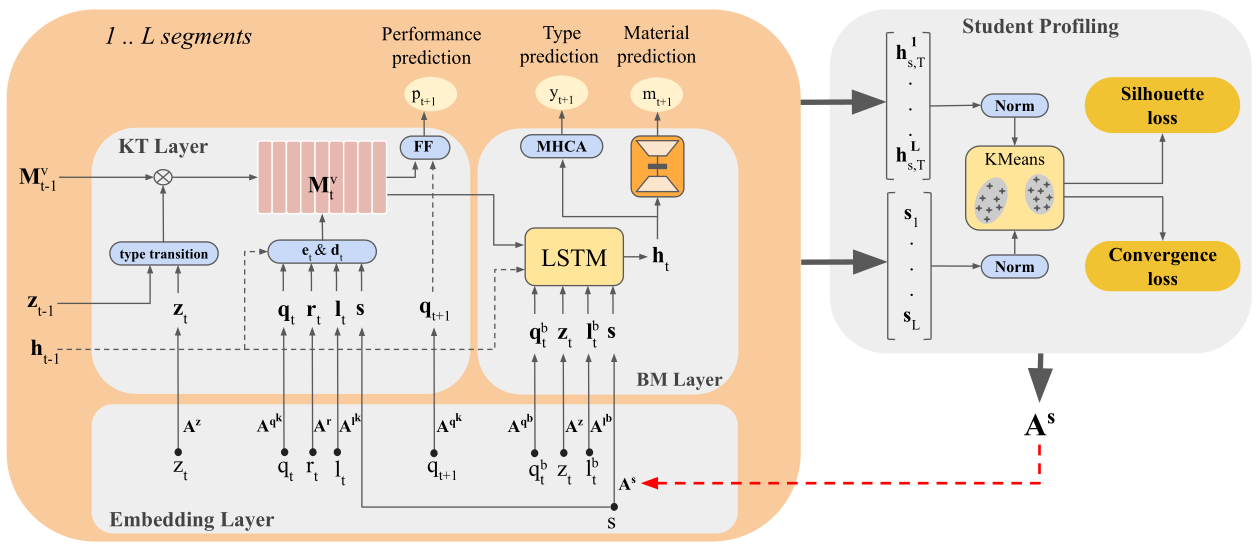
\includegraphics[width=0.8\textwidth]{The proposed model architecture for KMaP.png}
    \caption{Original KMaP model architecture (from \cite{hashemifar2025personalized}). Our enhanced framework builds upon this foundation by integrating: (1) LLM semantic embeddings in the material representation layer, (2) adaptive forgetting mechanisms within the LSTM components, and (3) gated MoE architecture for dynamic student profiling in place of static clustering.}
    \label{fig:architecture}
\end{figure}

\subsection{Innovation 1: Semantic Embeddings with LLMs}
\textbf{Implementation Strategy:} We replace traditional categorical encodings with 768-dimensional semantic representations from sentence-BERT \cite{reimers2019sentence}. We will pre-process all material texts to generate these embeddings offline. The resulting dense vectors will be concatenated with KMaP's existing categorical features and fed into the model's embedding layer, creating a hybrid representation.
\textbf{Justification:} Sentence-BERT has demonstrated superior performance in capturing semantic similarity \cite{reimers2019sentence}. This approach enables the model to recommend materials based on deeper conceptual understanding rather than superficial categorical matches, addressing a key limitation in current systems.

\subsection{Innovation 2: Adaptive Forgetting Gates}
\textbf{Implementation Details:} Inspired by cognitive science \cite{ebbinghaus1885memory,wixted2004psychology}, particularly the testing effect \cite{karpicke2008critical}, we implement learnable gating functions to model personalized knowledge decay. The forgetting gate $f_t$ is defined as:
\begin{equation}
    f_t = \sigma(W_f \cdot [h_t, \Delta t, d_m, p_s] + b_f)
\end{equation}
where the gate is conditioned on the current hidden state ($h_t$), time since last interaction ($\Delta t$), material difficulty ($d_m$), and a student-specific forgetting profile ($p_s$). The profile $p_s$ will be a learnable embedding vector, initialized by clustering students based on their historical interaction patterns.
\textbf{Justification:} Psychological research shows that forgetting patterns vary by individual and content \cite{wixted2004psychology,murre2015replication}. Our adaptive mechanism, informed by recent computational models \cite{sha2024forgetting,wang2024personalized}, moves beyond fixed decay rates to make more accurate long-term predictions about knowledge retention and optimize review timing.

\subsection{Innovation 3: Dynamic Profiling with Gated MoE}
\textbf{Architecture Design:} To overcome the limitations of static student profiles, we employ a gated Mixture-of-Experts (MoE) architecture \cite{shazeer2017outrageously,fedus2022switch,shelhamer2022mixture}. The model will consist of 4-6 specialized expert networks (small feed-forward networks) to capture distinct behavioral patterns. A lightweight, attention-based gating network will take the student's current context (e.g., recent performance, session length) and compute a soft assignment weight for each expert. The final output is a weighted sum of the expert outputs:
\begin{equation}
    y = \sum_{i=1}^{N} G(x)_i \cdot E_i(x)
\end{equation}
where $G(x)$ is the gating function and $E_i(x)$ are the expert networks.
\textbf{Justification:} Static profiling is inadequate for the dynamic nature of student learning. MoE architectures are proven for handling heterogeneous and evolving user behaviors in recommender systems and multi-task learning \cite{zou2025multi,ma2018modeling}, including large-scale industrial applications like YouTube video recommendations \cite{zhao2019recommending}. This allows our model to adapt to individual learning preferences and behavioral shifts in real-time.

\subsection{Integration and Training}
\textbf{Multi-task Learning Framework:} The model will be trained end-to-end using a multi-task loss function. This loss will be a weighted sum of a primary cross-entropy loss for knowledge tracing, a contrastive loss for material prediction, and auxiliary losses designed to guide the forgetting and MoE components. We will employ a progressive training strategy inspired by curriculum learning \cite{bengio2009curriculum}: first, train the baseline KMaP model; then, sequentially unfreeze and fine-tune each of the three innovative components. This staged approach ensures stable convergence and allows for clear ablation studies to validate each component's contribution.

\textbf{Evaluation Protocol:}
\begin{itemize}
    \item \textbf{Datasets:} EdNet (primary), Junyi Academy (validation).
    \item \textbf{Baselines:} Original KMaP, DKT, AKT, SAKT.
    \item \textbf{Metrics:} MRR, precision@k, AUC, behavioral consistency scores.
    \item \textbf{Statistical Testing:} Paired t-tests for significance validation.
    \item Target inference time within 100ms for practical deployment.
\end{itemize}

% Future Plan
\section{Project Plan}

The project follows a systematic 12-week implementation plan with four distinct phases, as illustrated in Figure \ref{fig:gantt_timeline}. The timeline ensures systematic development from foundation setup through final evaluation and documentation.

\begin{figure}[p]
    \centering
    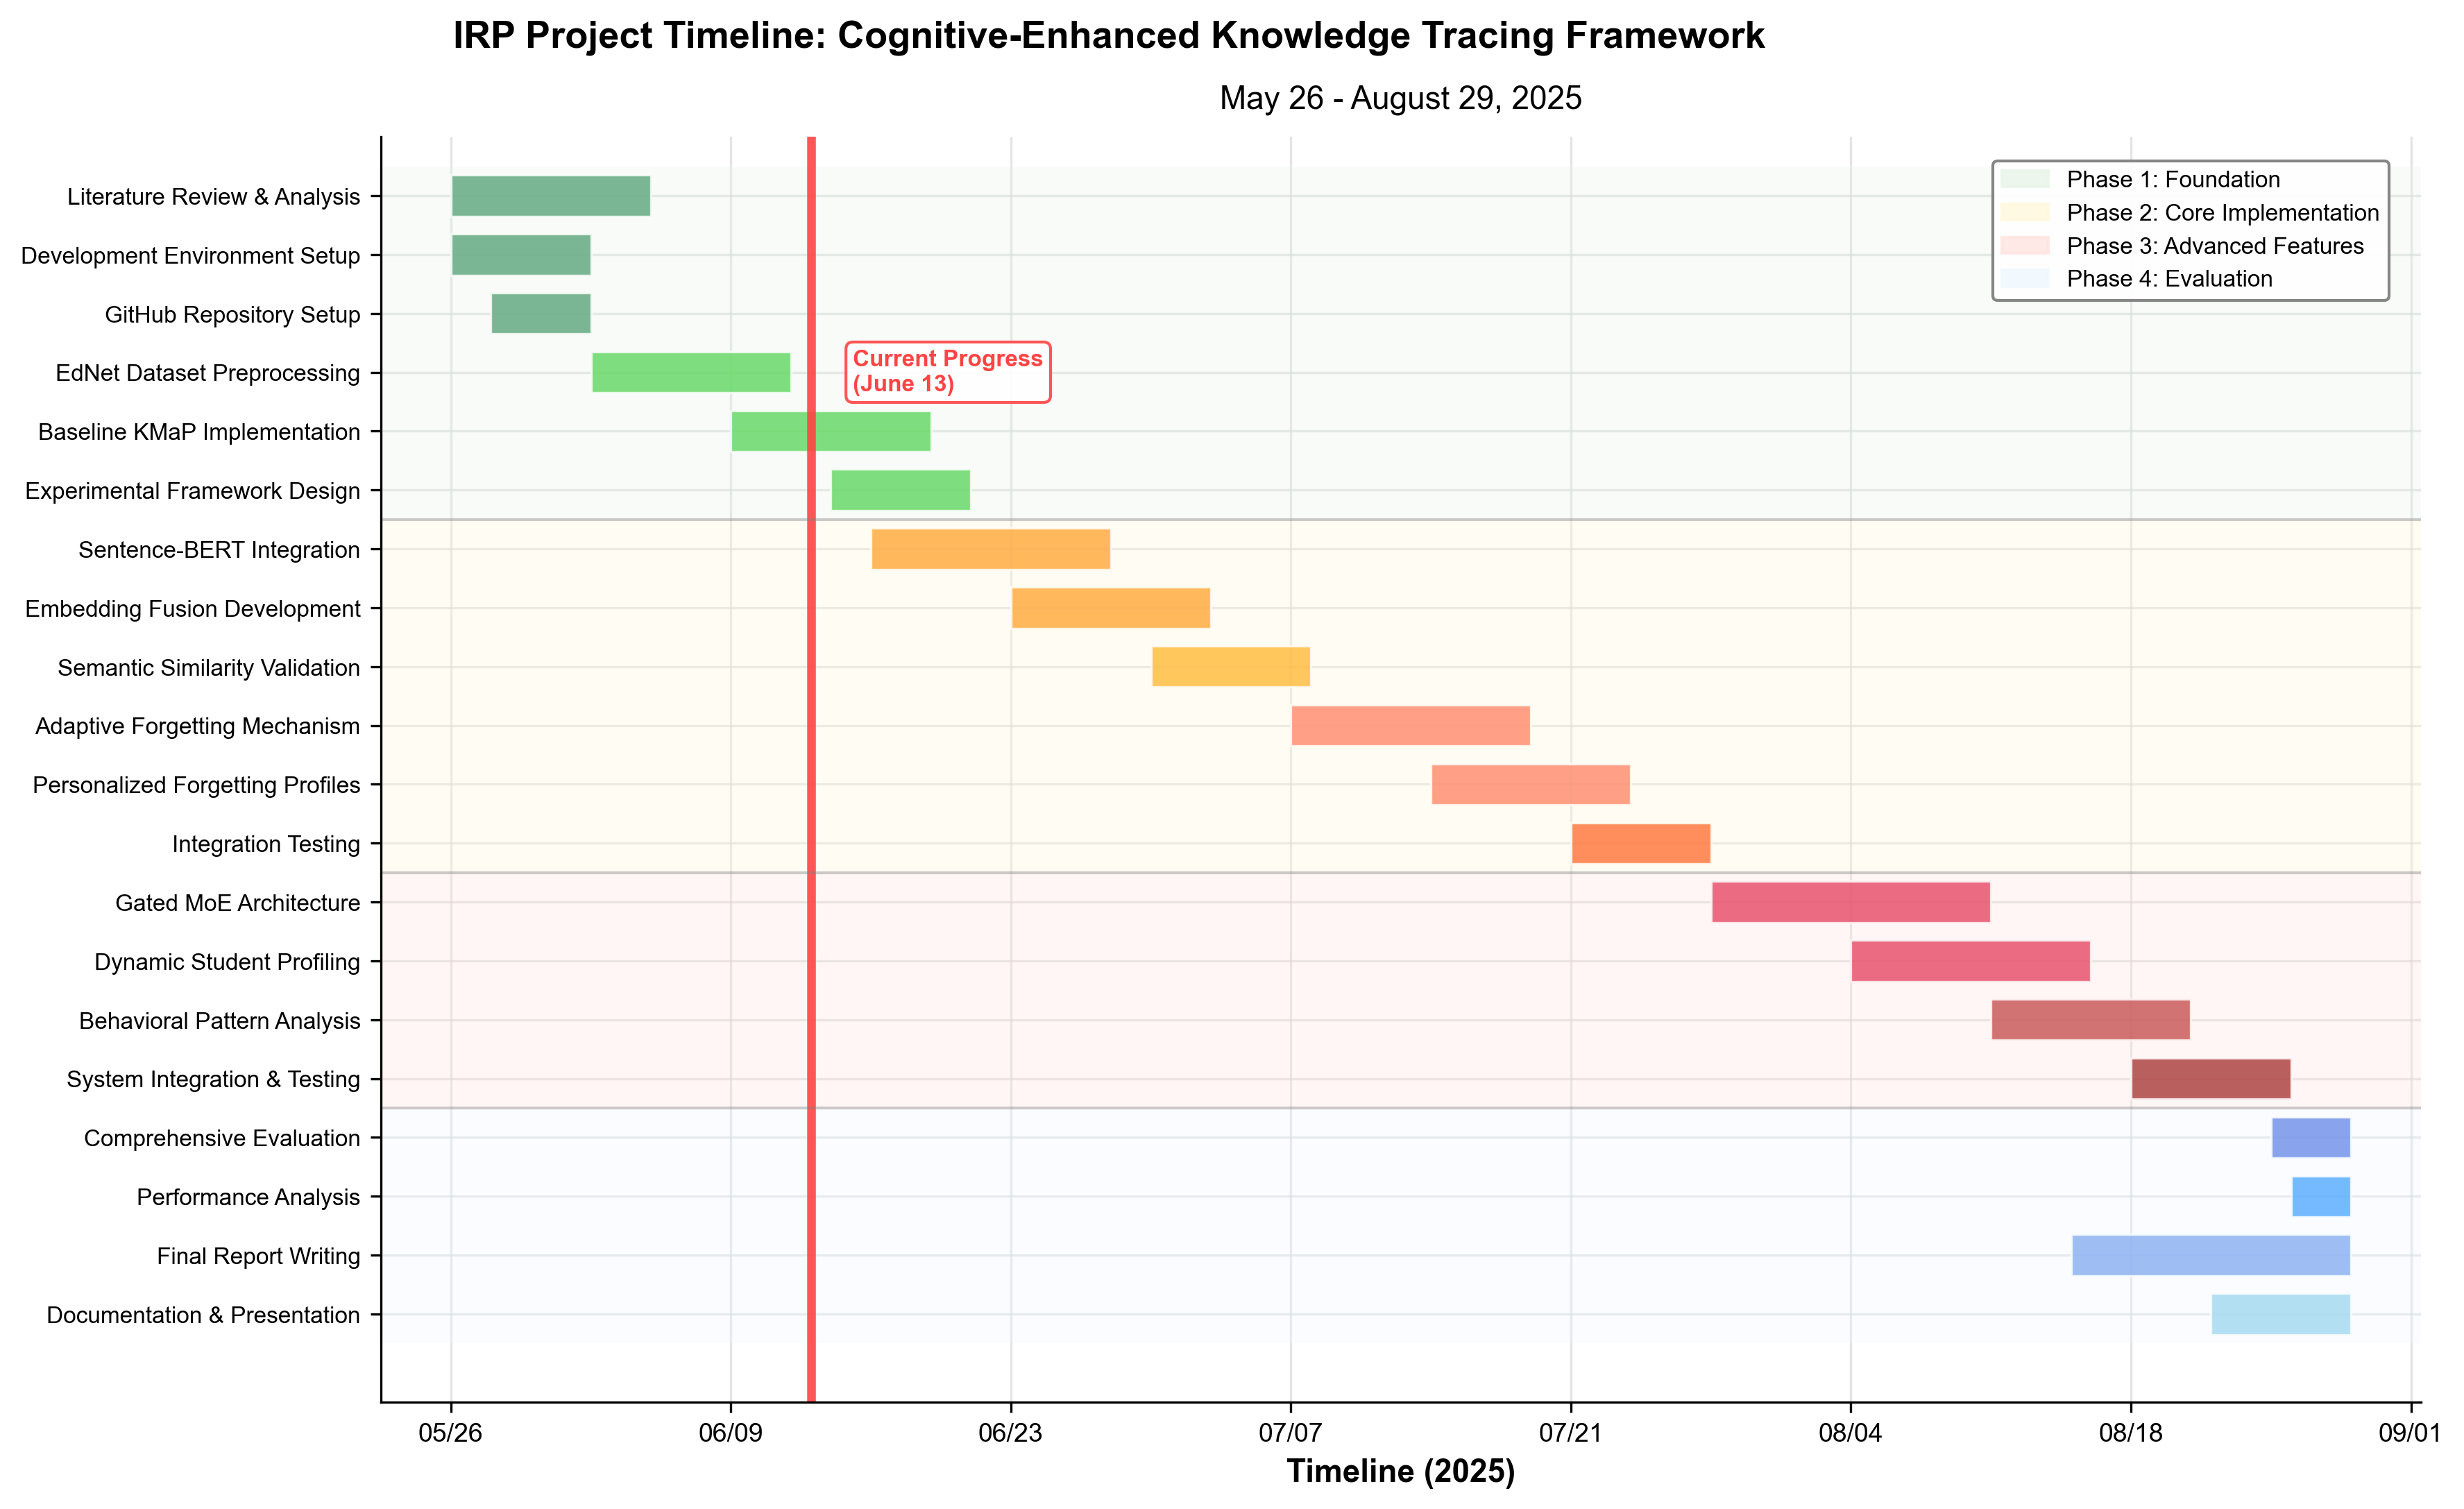
\includegraphics[angle=90, width=0.95\textwidth]{project_gantt_chart.png}
    \caption{Project timeline showing four-phase implementation with milestone tracking.}
    \label{fig:gantt_timeline}
\end{figure}

The implementation strategy is designed for modularity and risk mitigation. Each of the three core innovations will be developed and validated in separate work packages before being integrated into the final framework. This approach simplifies debugging, allows for parallel development where feasible, and enables clear, incremental validation of each component's contribution to overall performance.

\textbf{Risk Mitigation Strategies:}
\begin{itemize}
    \item \textbf{Computational Complexity:} Pre-compute sentence-BERT embeddings offline; implement efficient batch processing and sparse MoE routing.
    \item \textbf{Model Convergence:} Use established initialization strategies for MoE; maintain fallback to simpler profiling if needed.
    \item \textbf{Performance Validation:} Implement incremental improvement tracking; prepare alternative optimization strategies if targets are not met.
    \item \textbf{Timeline Management:} Maintain a schedule buffer; design simplified fallback implementations for complex components.
\end{itemize}

\subsection{Supervision and Project Management}
\textbf{Meeting Schedule:} I will meet with my main supervisor Dr. Wenxia Yang weekly and with co-supervisor Dr. Deborah Pelacani Cruz monthly. All meetings will be conducted in person when possible, with camera-on video calls as backup. I will maintain an active role in discussions, present progress updates, and seek guidance on technical challenges.

\textbf{Version Control Strategy:} I commit to regular, meaningful commits to the IRP repository with descriptive messages. The repository will include:
\begin{itemize}
    \item Weekly commits of code development and experimental results
    \item Bi-weekly commits of report drafts and documentation updates  
    \item Detailed commit messages describing specific changes and progress
    \item Proper branching strategy for different development phases
    \item Regular backup of all project materials to ensure reproducibility
\end{itemize}

\textbf{Logbook Maintenance:} After each supervisory meeting, I will update the \texttt{logbook.md} file in the repository with meeting details, feedback received, and action items for the next period. This will serve as a transparent record of project evolution and supervisory engagement.

% References
\bibliographystyle{unsrt}
\bibliography{references}  % BibTeX references are saved in references.bib

\end{document}          
